\documentclass[a4paper, 11pt, spanish]{article}
%QUITA IDENTACIÓN
\setlength{\parindent}{0pt}

% ---------------- Paquetes de formato.
\usepackage[spanish]{babel} % Para codificar el texto.
\usepackage[top=70mm, bottom=30mm, left=18mm, right=18mm]{geometry} % Para modificar el tamaño de las hojas.
\usepackage{fancyhdr} % Para poner la institución, dpto y curso arriba.
\usepackage{parallel} % Para escribir en columnas (Poner los integrantes a la derecha).
\usepackage[firstpage=false]{background} % Para poner el logo de la U arriba en todas las páginas.
\usepackage{enumerate} % Para poder enumerar como a), b), etc.
\usepackage[utf8]{inputenc} % Para usar acentos en vez de \'.

% ---------------- Paquetes graficos.
\usepackage{graphicx} % remove the demo option.
\usepackage{tikz}
\usepackage{caption}
\usepackage{subcaption} % Para usar sub-figuras

% ---------------- Paquetes matematicos.
\usepackage{amsmath} % Para poder hacer N^o y se vea bonito.
\usepackage{amsthm} % Fonts matematicos.
\usepackage{amssymb} % Para usar \therefore
\usepackage{commath} % Para usar \abs y \norm

% ---------------- Paquetes 'computines'.
\usepackage{listings} % Para escribir codigo y que se vea bonito.
\usepackage[% Descomentar las opciones a usar.
spanish,
%boxed, % Encierra los algoritmos en un cuadro.
boxruled, % Encierra los algoritmos en un cuadro colocando el titulo al comienzo.
%ruled, % Coloca una linea al comienzo y otra al final del algoritmo. El titulo de este queda al comienzo del algoritmo.
%algoruled, % Lo mismo que el anterior pero mas espaciado.
%tworuled, % Como ruled pero sin una linea al comienzo.
%algochapter, % Los algoritmos se enumeran segun capitulo.
%algopart, % Los algoritmos se enumeran por partes.
%figure, % Los algoritmos son considerados figuras (y por ende salen en \listoffigures).
%linesnumbered, % Enumera las lineas.
longend % Los end son para cada ciclo, por ejemplo endif para los if-else.
]{algorithm2e}

% ---------------- Paquetes miscelaneos.
%\usepackage{lipsum} % Para hacer placeholders.
\usepackage{bohr} % Para dibujar atomos.

% ---------------- Comando mas corto para insertar figuras. Ojo que deben estar guardadas en ./img/
% \fig{name}{width}{height}{caption}
\newcommand{\fig}[4]{%
	\begin{figure}[!htbp]
		\centering
		\includegraphics[width=#2, height=#3]{img/#1}
		\caption{#4}
	\end{figure}
}
% ejemplo:
%\fig{nombre_imagen.png}{10cm}{5cm}{Titulo de la imagen}

%%% Ejemplo para poner dos imagenes juntas, lado a lado

%\begin{figure}[!ht]
%\centering
%\begin{subfigure}{.5\textwidth}
%  \centering
%  \includegraphics[width=10cm, height=8cm]{img/curva0f1.pdf}
%  \caption{Curva de nivel 0 de $F_{1}$.}
%  \label{fig:sub1}
%\end{subfigure}%
%\begin{subfigure}{.5\textwidth}
%  \centering
%  \includegraphics[width=10cm, height=8cm]{img/curva0f2.pdf}
%  \caption{Curva de nivel 0 de $F_{2}$.}
%  \label{fig:sub2}
%\end{subfigure}
%\caption{Curvas de nivel 0 de $F_{1}$ y $F_{2}$}
%\label{fig:test}
%\end{figure}

%%Ejemplo figura Normal
%\begin{figure}[h]
%\centering
%\includegraphics[scale=0.7]{ex1}
%\caption{Disposición geométrica experimento 1, se puede notar en rojo la línea en que se efectuaron las mediciones hechas} 
%\end{figure} 

% ---------------- Comando para hacer itemes
% \Solution{pregunta}{solucion}
\newcommand{\Solution}[2]{%
	\item #1 \vspace{0.2cm}
	\textbf{Soluci\'on:} #2
}
% \Demonstration{pregunta}{demostracion}
\newcommand{\Demonstration}[2]{%
	\item #1 \vspace{0.2cm}
	\begin{proof}
		#2	
	\end{proof}
}

% ---------------- Opciones de algortihm2e
\SetKw{KwRequire}{Require:}

% ---------------- Opciones de background.
\SetBgColor{black}
\SetBgScale{1}
\SetBgOpacity{1}
\SetBgAngle{0}
\SetBgContents{%
	\begin{tikzpicture}[remember picture,overlay]
		\node at (-8.0,0.746\textheight) {\includegraphics[height=18mm,width= 0.155\textwidth]{img/LogoUIngenieria.png}};
	\end{tikzpicture}
}

% ---------------- Creacion de institucion, departamento y curso.
\fancyheadoffset[L]{-2cm}
\fancyhead[L]{\footnotesize{\textbf{\textsf{Universidad de Chile \\ Facultad de Cs. F\'isicas y Matem\'aticas \\ Departamento de F\'isica \\ Métodos Númericos : FI3104-1}}}}
\renewcommand{\headrulewidth}{0pt}
\setlength{\voffset}{-3cm}

\pagestyle{fancy} % Estilo de las páginas

\begin{document}

\pagenumbering{gobble} % Quita el numero de las paginas (y las resetea a 1)

\clearpage

\thispagestyle{fancy}
\vspace*{6.5cm} % Espacio vertical para posicionar bien el título (En una de esas esto se puede optimizar para que no sea tan a la fuerza bruta).

% ---------------- Titulo.
\begin{center}
	\Large{\textbf{\textsf{Informe Tarea 4}}} \\
	\huge{\textbf{\textsf{Resolución de Sistemas Lineales}}}
\end{center}

\vspace*{7.5cm}

% ---------------- Integrantes, profes, etc.
\begin{Parallel}{1cm}{7.5cm}
	\ParallelRText{%
		\begin{flushright} % Tira el texto hacia la derecha.
			\large{%
				\textsf{%
					\begin{tabular}{rl}
						Alumno: &
							\begin{tabular}[t]{@{}l@{}}
								Bruno Quezada
							\end{tabular} \\
						Profesore: & 
							\begin{tabular}[t]{@{}l@{}}
						 		Valentino González
							\end{tabular} \\
						Auxiliares: &
							\begin{tabular}[t]{@{}l@{}}
								José Vines. \\
								Jou-Hui Ho.
							\end{tabular} \\	 
					\end{tabular} \\
					Fecha: \today
				}
			}
		\end{flushright}
	}
\end{Parallel}

\clearpage

\pagenumbering{arabic} % Numeros de pagina Arabicos (y los resetea a 1)

\newpage

\tableofcontents % Indice. Descomente para usar.
%\listoffigures % Lista de figuras. Descomente para usar.
%\listoftables % Lista de tablas. Descomente para usar.

\newpage

\section{Introducci\'on}
En esta pregunta se busca resolver un sistema lineal, a través de distintos métodos, para poder evaluar las distintas resoluciones y sus desempeños. Para este caso resolveremos un sistema lineal que representa las tensiones que existen en un sistema de 12 cuerdas como se puede ver en la figura \ref{cuerdas}.\\

Para ello, se plantearon las ecuaciones de equilibrio de fuerzas y con distintos métodos se resolverá el sistema
\begin{figure}[h]
\centering
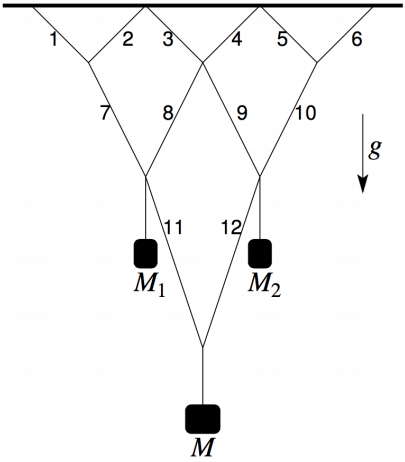
\includegraphics[scale=0.7]{cuerdas.png}
\caption{Sistema de cuerdas a resolver}
\label{cuerdas} 
\end{figure} 

\section{Procedimiento}
En primera instancia es necesario plantear el problema en forma matricial, de la forma:
\begin{equation}
A \cdot T = m
\end{equation}

En donde las columnas de $A$ representan las relaciones que tienen las distintas tensiones de las cuerdas para cada nodo, $\Sigma F$ para la componente x e y del problema, $T$ corresponde al vector de tensiones de cada cuerda y $m$ representa a los pesos que se le agrega al sistema para que esté tensionado.\\
Al plantear el problema de esta manera se está resolviendo en forma matricial la segunda ley de Newton, $\Sigma F = ma $.\\
Los métodos para encontrar $T$ fueron:\\
\textbf{Método 1: reducción de Gauss} se utiliza el método \textit{solve()} del paquete \textit{scipy.linalg}, el cual resuelve el sistema a través de la reducción de Gauss. Esta reducción consiste en pivotear la matriz A hasta que quede con una diagonal de $1$ y triangular superior. Con esta clase de matriz es muy fácil el despeje de las distintas tensiones de las cuerdas.\\

\textbf{Método 2: descomposición LU} se utiliza el método \textit{solve \_ triangular} del módulo \textit{scipy.linalg} el cual descompone la matriz A en dos matrices triangulares, una superior y otra inferior de la forma que:
\begin{equation}
A = L \cdot U
\end{equation}
Con esta descomposición se encuentra $T$ resolviendo las siguientes operaciones matriciales:
\begin{equation*}
U \cdot x = y 
\end{equation*}
\begin{equation}
y \cdot B = T
\end{equation}
\\

\textbf{Método 3: invertir $A$}: Se calcula la inversa de la matriz $A$ con la función \textit{inv()} del módulo \textit{scipy.linalg} y se premultiplica en la ecuación:
\begin{equation}
A^{-1} \cdot A \cdot T = A^{-1} \cdot b \Rightarrow T = A^{-1} \cdot b
\end{equation}


\section{Resultados}
En la figura \ref{dist} se presenta la distribución de tensiones de las cuerdas para $M1 = 1.5[kg]$, em la figura \ref{tmax} se presenta la cuerda que posee la máxima tensión (derecha) y la máxima tensión en Newton (izquierda). En la tabla 1 se presentan los distintos tiempos que le tomó al computador resolver el sistema, calculados con el comando \textit{timeit}, para calcular el tiempo de cómputo del tercer método se tuvo que realizar varias veces ya que la desviación estándar era muy grande para las primeras iteraciones.\\

\begin{figure}[h]
\centering
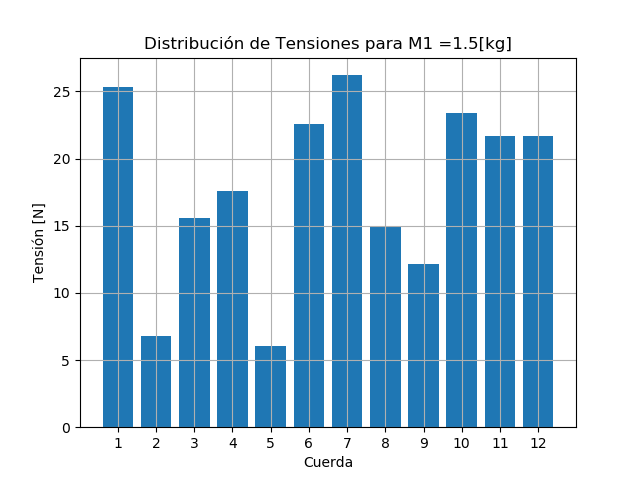
\includegraphics[scale=0.7]{dist_tensiones.png}
\label{dist}
\caption{Distibución de tensiones en las cuerdas para $M1 = 1.5[kg]$} 
\end{figure} 

\begin{figure}[h]
\centering
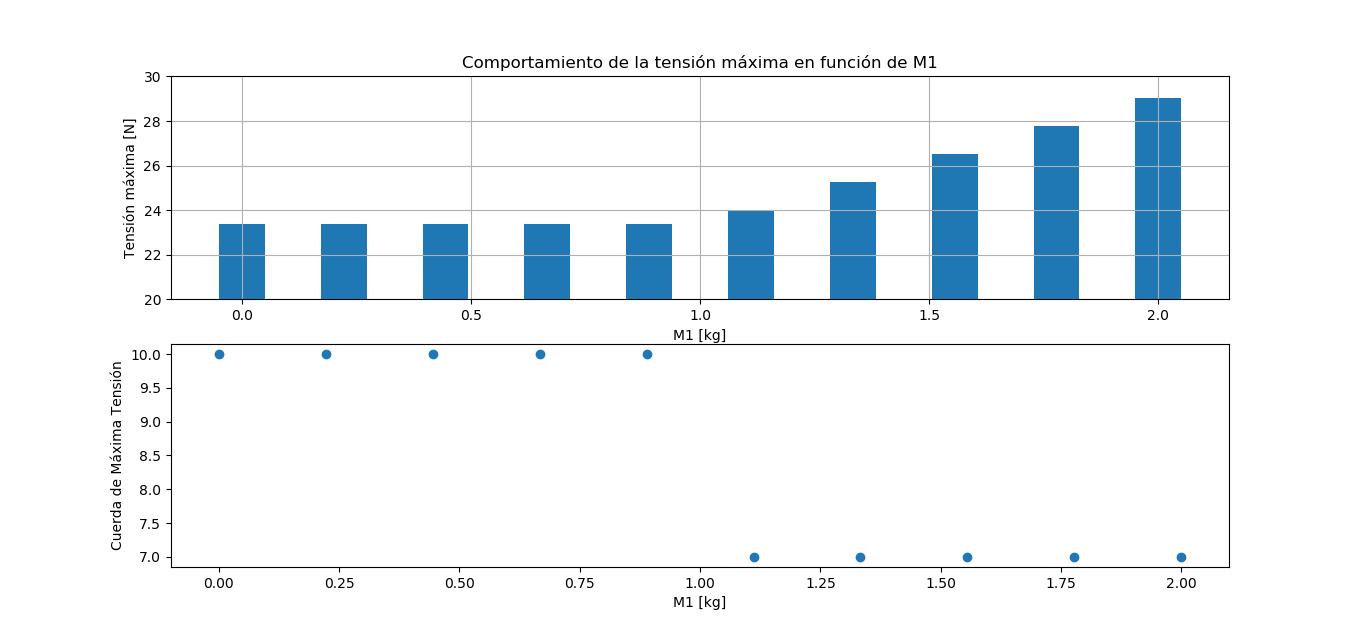
\includegraphics[scale=0.4]{tensionesmaximas_0.png}
\label{tmax}
\caption{en la izquierda las tensiones máximas para distintos valores de M1 y en la derecha el índice de la cuerda} 
\end{figure} 

\begin{table}[h]
\centering
\begin{tabular}{|l|l|}
\hline
\multicolumn{2}{|c|}{\textbf{Tiempo Algoritmo}}               \\ \hline
Método 1: reducción de Gauss & $313  [\mu s] \pm 179 [\mu s]$ \\ \hline
Método 2: descomposición LU  & $209 [\mu s] \pm 9 [\mu s]$    \\ \hline
Método 3: inversión de A     & $93 [\mu s] \pm 1 [\mu s]$     \\ \hline
\end{tabular}
\end{table}

 
\section{Conclusiones y Discusi\'on}

Se considera que se logró resolver en forma exitosa el problema propuesto. A través de los distintos métodos de resolución se lograron resultados consistentes, por lo que fueron bien implementados.\\
Una dificultad importante de esta clase de problemas es el planteo de la matriz A, es necesario asignar las variables de forma inteligente y ser consistente con el sistema de referencia utilizado para no cometer errores. Un mal planteo de la matriz A generará que se esté representando otro sistema al que se quiere resolver.\\

Es de gran sorpresa para el autor que el método de la inversión tuvo el mejor rendimiento. En el caso general se considera muy costoso computacionalmente invertir matrices, en este caso la matriz $A$ es sólo de $12x12$ y es de tipo sparse (muchos elementos nulos), estas características particulares de $A$ reducen el tiempo necesario para determinar su inversa.\\

Como existen muchos métodos para resolver problemas lineales, es importante conocer las ventajas y desventajas de cada uno de ellos, para poder implementar el método más adecuado. En este caso la inversión tiene la ventaja de que una vez obtenida $A{-1}$ sólo es necesario hacer una multiplicación matricial para encontrar $T$, por lo que si se quiere estudiar el comportamiento de un sistema frente a variaciones de sus componentes del vector $b$ este método es más adecuado. Para resolver un problema con una matriz $A$ grande y que no se quiera variar los parámetros de $b$, es más conveniente usar la descomposición LU, ya que tuvo un mejor desempeño en comparación a la reducción de Gauss.

\end{document}
